\section{Resultados y Análisis}
En esta sección presentaremos y analizaremos los resultados obtenidos al correr los distintos test propuestos.
Para ello correremos los mismos con una iteración de 100 repeticiones sobre los host de las siguientes universidades.

\subsection{Universidad de Tokyo}
El host de destino de la universidad de Tokyo sera el dominio ``www.u-tokyo.ac.jp'' cuya IP es ``210.152.135.178''. El host de la universidad de Tokyo se encuentra ubicado la ciudad de Tokyo, Japón. El origen sera un host ubicado en la Ciudad de Buenos Aires, Argentina utilizando como isp a Telecentro.

\subsubsection{Datos}

Los datos obtenidos para este caso fueron los siguientes:

\begin{table}[H]
    \begin{center}
        \begin{tabular}{| r | r | r | r | r |}
  \hline
  {\bf TTL} & \multicolumn{1}{|c|}{\bf IP} & {\bf E(RTT) (ms)} & {\bf S(RTT) (ms)} & {\bf $\Delta$RTT (ms)}\\
  \hline
\hline 1  & 192.168.10.1 & 0.414 & 0.025 & 0.414\\
\hline 2  & 10.20.64.1 & 9.588 & 2.179 & 9.174\\
\hline 3  & 200.115.194.173 & 9.709 & 2.050 & 0.121\\
\hline 4  & 208.178.195.210 & 11.823 & 2.660 & 2.114\\
\hline 5  & 208.178.195.209 & 10.154 & 3.919 & 0.000\\
\rowcolor{blue!25}\hline 6  & 64.212.107.98 & 140.102 & 2.736 & 129.948\\
\hline 7  & 129.250.3.172 & 141.972 & 6.459 & 1.870\\
\hline 8  & 129.250.2.219 & 165.020 & 5.163 & 23.048\\
\hline 9  & 129.250.7.69 & 174.848 & 10.839 & 9.828\\
\rowcolor{blue!25}\hline 10  & 129.250.2.177 & 289.040 & 10.215 & 114.191\\
\hline 11  & 129.250.6.144 & 286.955 & 9.046 & 0.000\\
\hline 12  & 61.200.80.218 & 281.767 & 6.327 & 0.000\\
\hline 13  & 158.205.192.173 & 287.145 & 8.005 & 5.378\\
\hline 14  & 158.205.192.86 & 300.318 & 5.018 & 13.173\\
\hline 15  & 158.205.121.250 & 299.293 & 22.325 & 0.000\\
\hline 16  & 154.34.240.254 & 287.327 & 2.431 & 0.000\\
\hline 17  & 210.152.135.178 & 300.554 & 3.888 & 13.227\\
\hline
        \end{tabular}
        \caption{$\overline{RTT}$, $\sigma$RTT y $\Delta$RTT para la ruta utilizada para llegar www.u-tokyo.ac.jp}
        \label{table:tokyo} 
    \end{center}
\end{table}

Analizando la información aportada por la tabla \ref{table:tokyo} podemos notar que tanto el salto 6 como 10 sobresalen por sobre el resto en cuanto a sus tiempos de $\Delta$RTT. 

\subsubsection{RTT y $\Delta$RTT}

\begin{figure}[H]
    \begin{center}
        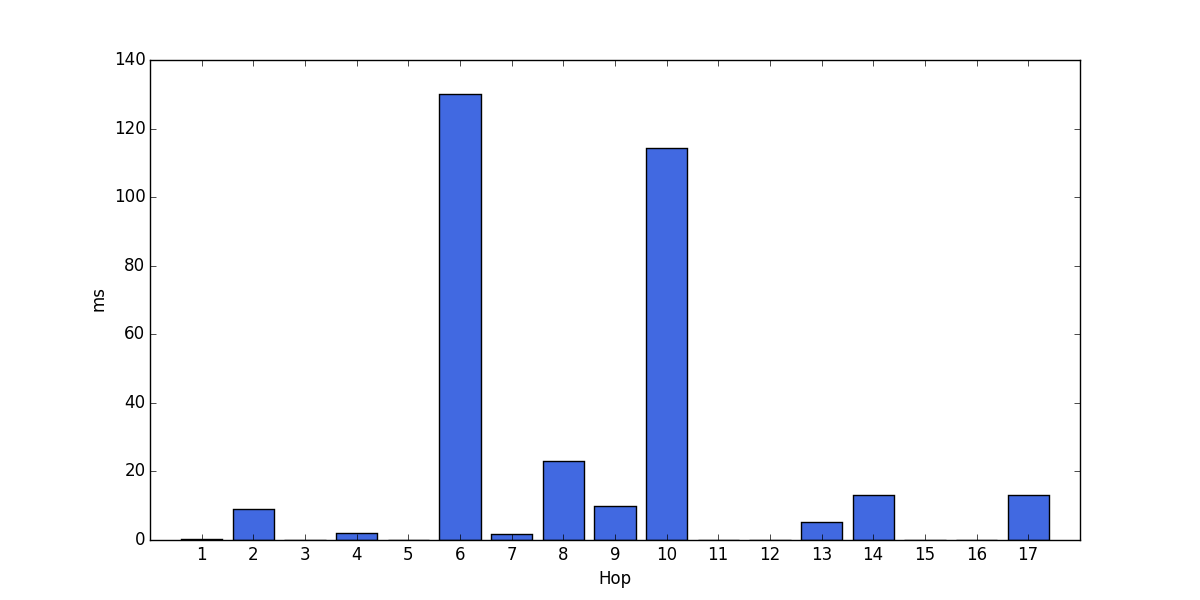
\includegraphics[width=1\textwidth]{data/rtt-tokyo-bar.png}
        \caption{www.u-tokyo.ac.jp - $\Delta$RTT}
        \label{histo:tokyo}
    \end{center}
\end{figure}

\begin{figure}[H]
    \begin{center}
        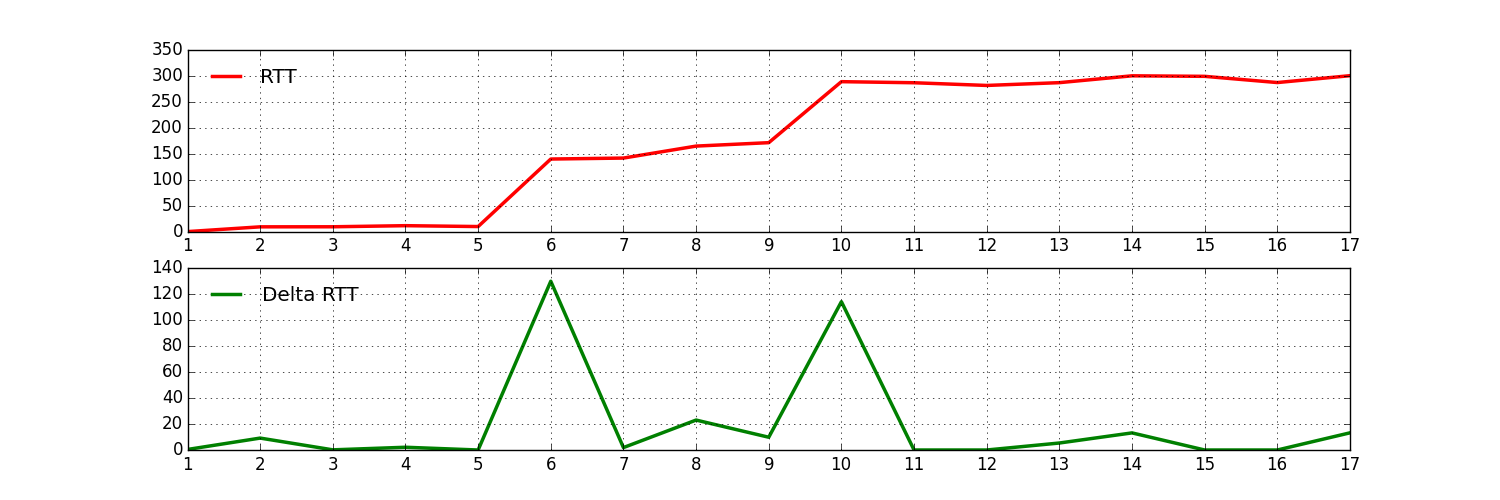
\includegraphics[width=1\textwidth]{data/rtt-tokyo-lines.png}
        \caption{www.u-tokyo.ac.jp - RTT y $\Delta$RTT}
        \label{lines:tokyo}
    \end{center}
\end{figure}

Tanto en la figura \ref{histo:tokyo} como en la figura \ref{lines:tokyo} podemos comprobar los que habíamos notado en la tabla \ref{table:tokyo}. Esto es que tanto el salto 6 como 10 se destacan por sobre el resto. En caso de existir algún enlace submarino seguramente este se correspondería con alguno de estos saltos. Esto lo analizaremos en las siguientes secciones.

\subsubsection{Test de Grubbs}\label{tokyo:grubbs}

Previo a correr el test de Grubbs corrimos un test de normalidad sobre la distribución de $\Delta$RTT obteniendo los siguientes resultados:

\begin{itemize}
\item \textbf{z-score: 21.762}
\item \textbf{p-value: 0.002}
\end{itemize}

De los resultados obtenidos deducimos entonces que la distribución de los $\Delta$RTT no tiene una distribución Normal, igualmente como mencionamos en la sección \ref{desarrollo:stats} correremos el test de Grubbs a fin de corroborar luego si encuentra los enlaces submarinos de todas formas.\\
Los resultados obtenidos fueron los siguientes outliers:

\begin{itemize}
\item 64.212.107.98
\item 129.250.2.177
\end{itemize}

\subsubsection{Geolocalización}

\begin{table}[H]
    \begin{center}
        \begin{tabular}{| r | r | c | c |}
  \hline
  {\bf TTL} & \multicolumn{1}{|c|}{\bf IP} & {\bf DNS} & {\bf Ubicación}\\
  \hline
\hline 1  & 192.168.10.1 & rig0.tuxhome.com.ar(ip privada) &\\
\hline 2  & 10.20.64.1 & no disponible(ip privada) &\\
\hline 3  & 200.115.194.173 & cpe-200-115-194-173.telecentro-reversos.com.ar & Buenos Aires, Argentina\\
\hline 4  & 208.178.195.210 & global-crossing-argentina-s-a.xe-0-1-0.ar3... & Buenos Aires, Argentina \\
\hline 5  & 208.178.195.209 & xe-0-1-0.ar3.eze1.gblx.net & Buenos Aires, Argentina \\
\rowcolor{blue!25}\hline 6  & 64.212.107.98 & no disponible  & Los Angeles, Usa\\
\hline 7  & 129.250.3.172 & ae-4.r21.miamfl02.us.bb.gin.ntt.net & Miami, Usa \\
\hline 8  & 129.250.2.219 & ae-4.r22.dllstx09.us.bb.gin.ntt.net & Dallas, Usa\\
\hline 9  & 129.250.7.69 & ae-5.r22.lsanca07.us.bb.gin.ntt.net & Los Angeles, Usa\\
\rowcolor{blue!25}\hline 10  & 129.250.2.177 & ae-0.r21.osakjp02.jp.bb.gin.ntt.net & Houston, Usa\\
\hline 11  & 129.250.6.144 & ae-5.r23.osakjp02.jp.bb.gin.ntt.net & Osaka, Japan\\
\hline 12  & 61.200.80.218 & xe-1-1-10.r23.osakjp02.jp.ce.gin.ntt.net & Osaka, Japan\\
\hline 13  & 158.205.192.173 & ae0.ostcr01.idc.jp & Tokyo, Japan\\
\hline 14  & 158.205.192.86 & no disponible  & Tokyo, Japan\\
\hline 15  & 158.205.121.250 & po2.l321.fk1.eg.idc.jp & Tokyo, Japan\\
\hline 16  & 154.34.240.254 & no disponible & Tokyo, Japan\\
\hline 17  & 210.152.135.178 & www.u-tokyo.ac.jp & Tokyo, Japan\\
\hline
        \end{tabular}
        \caption{Ruta utilizada para llegar www.u-tokyo.ac.jp con la ubicación de los diferentes saltos por los que se pasa. Se encuentran resaltados los saltos distinguidos calculados en la sección \ref{tokyo:grubbs}}
        \label{table:tokyo} 
    \end{center}
\end{table}

En la tabla \ref{table:tokyo} notamos que el salto 10 figura ubicado en Houston, Estados Unidos, sin embargo dado el $\Delta$RTT de este salto que hizo que sea distinguido como outlier en la la sección \ref{tokyo:grubbs} y su DNS reverso ``ae-0.r21.osakjp02.jp.bb.gin.ntt.net'' inferimos que es un error en las bases de datos de geolocalización y que ese salto se encuentra efectivamente ubicado en Osaka, Japon. Por este motivo al trazar el traceroute sobre el mapa de la figura \ref{mapa:tokyo} lo ubicamos en esta última localidad.

\begin{figure}[H]
    \begin{center}
        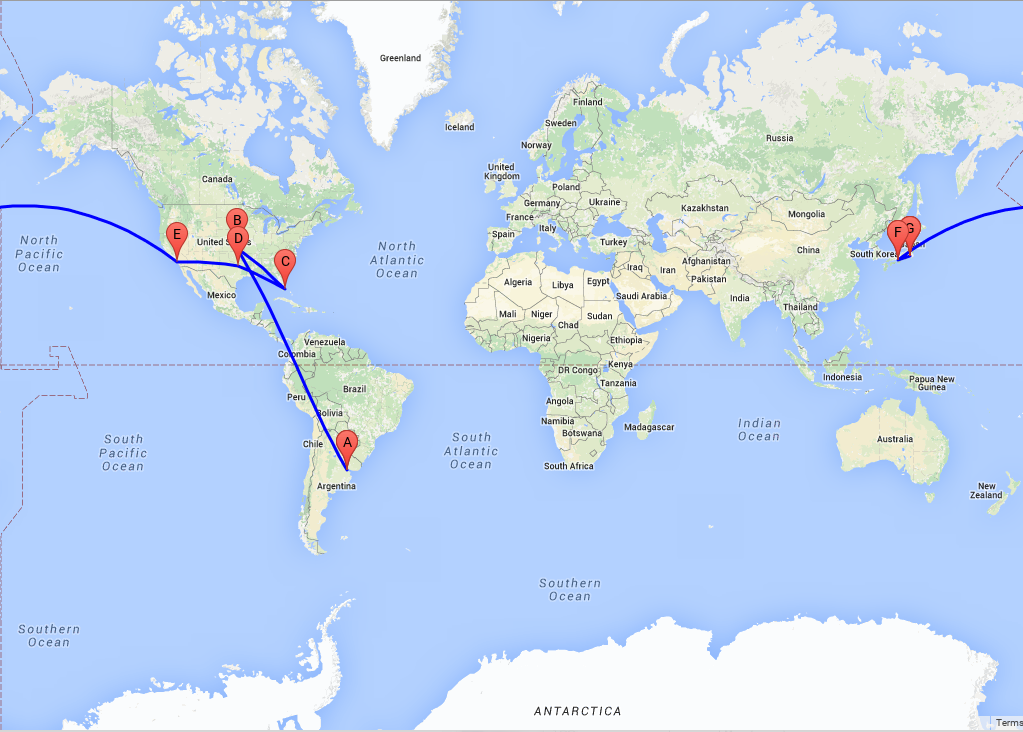
\includegraphics[width=1\textwidth]{data/mapa-tokyo.png}
        \caption{www.u-tokyo.ac.jp - Traceroute}
        \label{mapa:tokyo}
    \end{center}
\end{figure}

\subsection{Universidad de Pretoria}
El host de destino de la universidad de Pretoria sera el dominio ``www.up.ac.za'' cuya IP es ``5.10.110.85''. El host de la universidad de Pretoria se encuentra ubicado la ciudad de Pretoria, en Sudáfrica. El origen es un host ubicado en la Ciudad de Buenos Aires, Argentina utilizando como isp a Telecentro.

\subsubsection{Datos}

Los datos obtenidos para este caso fueron los siguientes:

\begin{table}[H]
    \begin{center}
        \begin{tabular}{| r | r | r | r | r |}
  \hline
  {\bf TTL} & \multicolumn{1}{|c|}{\bf IP} & {\bf E(RTT) (ms)} & {\bf S(RTT) (ms)} & {\bf $\Delta$RTT (ms)}\\
  \hline 
\hline 1  & 192.168.0.1 &  3.037 & 3.218 & 3.037\\
\rowcolor{blue!25}\hline 2  & 10.19.0.1 & 21.794 & 23.114 & 18.757\\
\hline 3  & 200.115.195.81 & 19.089 & 14.663 & 0.000\\
\hline 4  & 208.178.195.214 & 20.840 & 13.042 & 1.751\\ 
\hline 5  & 208.178.195.213 & 22.422 & 18.565 & 1.582\\ 
\rowcolor{blue!25}\hline 6  & 67.17.75.66 & 158.745 & 28.768 & 136.323\\ 
\hline 7  & 4.68.111.121 &  152.379 & 26.292 & 0.000\\ 
\rowcolor{blue!25}\hline 8  & 4.69.168.11 & 272.512 & 19.879 & 120.133\\ 
\hline 9  & 4.69.168.11 & 277.326 & 26.226 & 4.814\\ 
\rowcolor{blue!25}\hline 10  & 212.73.206.174 & 292.420 & 28.952 & 15.094\\ 
\hline 11  & 50.97.19.101 & 281.778 & 31.841 & 0.000\\ 
\hline 12  & 50.97.19.41 & 289.224 & 33.909 & 7.446\\ 
\hline 13  & 5.10.118.135 & 278.807 & 23.145 & 0.000\\ 
\hline 14  & 5.10.110.85 & 279.282 & 18.527 & 0.476\\ 
\hline
        \end{tabular}
        \caption{$\overline{RTT}$, $\sigma$RTT y $\Delta$RTT para la ruta utilizada para llegar www.up.ac.za}
        \label{table:pretoria} 
    \end{center}
\end{table}

Analizando la información aportada por la tabla \ref{table:pretoria} podemos notar que los saltos 2, 6, 8 y 10 sobresalen por sobre el resto en cuanto a sus tiempos de $\Delta$RTT. 

\subsubsection{RTT y $\Delta$RTT}

\begin{figure}[H]
    \begin{center}
        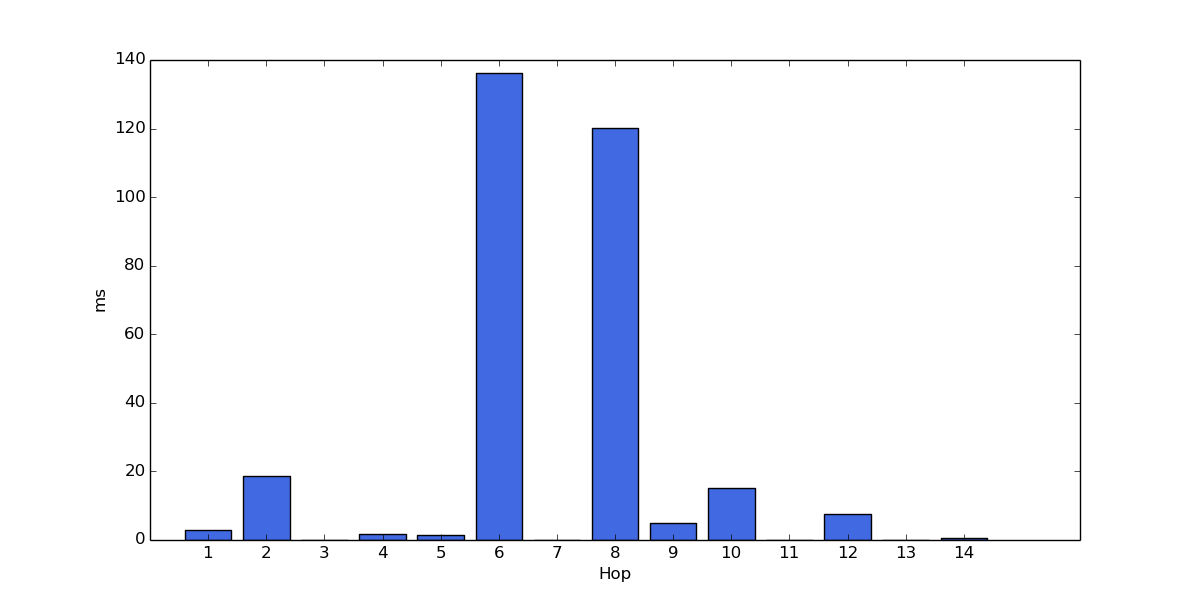
\includegraphics[width=1\textwidth]{data/rtt-pretoria-bar.png}
        \caption{www.up.ac.za - $\Delta$RTT}
        \label{histo:pretoria}
    \end{center}
\end{figure}

\begin{figure}[H]
    \begin{center}
        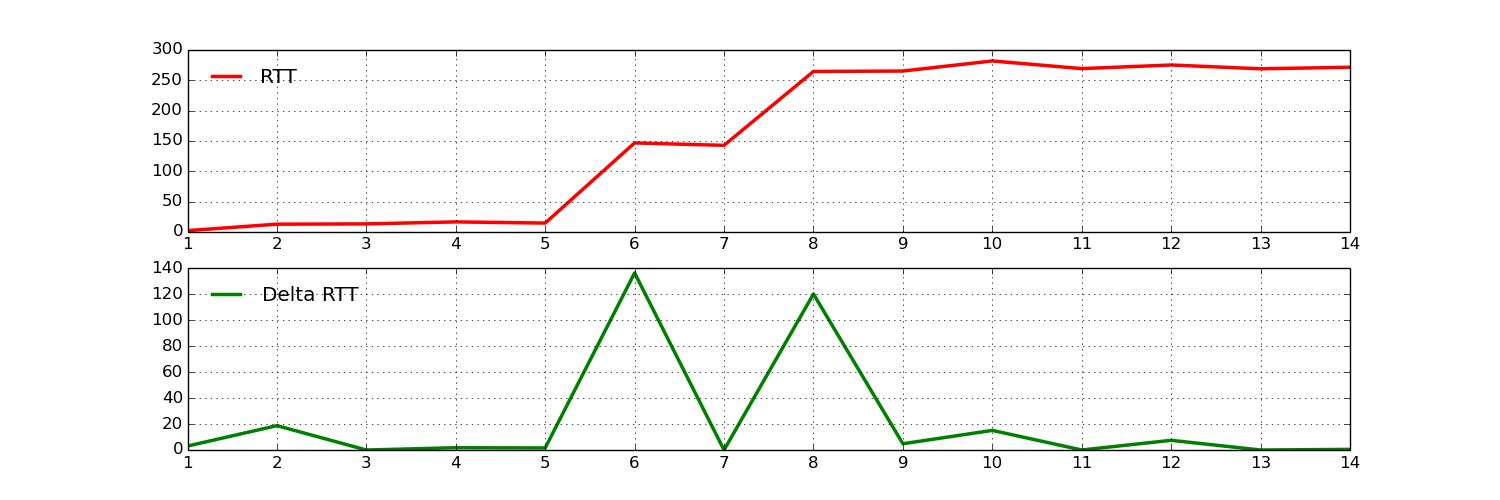
\includegraphics[width=1\textwidth]{data/rtt-pretoria-lines.png}
        \caption{www.up.ac.za - RTT y $\Delta$RTT}
        \label{lines:pretoria}
    \end{center}
\end{figure}

Tanto en la figura \ref{histo:pretoria} como en la figura \ref{lines:pretoria} podemos comprobar los que habíamos notado en la tabla \ref{table:pretoria}. Esto es que tanto los saltos 2, 6, 8 y 10 se destacan por sobre el resto. En caso de existir algún enlace submarino seguramente este se correspondería con alguno de estos saltos. Esto lo analizaremos en las siguientes secciones.

\subsubsection{Test de Grubbs}\label{pretoria:grubbs}

\subsubsection{Geolocalización}

\begin{table}[H]
    \begin{center}
        \begin{tabular}{| r | r | c | c |}
  \hline
  {\bf TTL} & \multicolumn{1}{|c|}{\bf IP} & {\bf DNS} & {\bf Ubicación}\\
  \hline
\hline 1  & 192.168.0.1 & (ip privada) & \\
\rowcolor{blue!25}\hline 2  & 10.19.0.1 & (ip privada) & \\
\hline 3  & 200.115.195.81 & cpe-200-115-195-81.telecentro-reversos.com.ar & Buenos Aires, Argentina\\
\hline 4  & 208.178.195.214 & global-crossing-argentina-s-a.xe-0-3-1.ar3.eze1.gblx.net & Buenos Aires, Argentina\\ 
\hline 5  & 208.178.195.213 & xe-0-3-1.ar3.eze1.gblx.net & Buenos Aires, Argentina\\ 
\rowcolor{blue!25}\hline 6  & 67.17.75.66 &  po3-20G.ar3.MIA2.gblx.net & Miami, USA\\ 
\hline 7  & 4.68.111.121 &  ae5.edge2.miami2.level3.net  & Miami, USA\\ 
\rowcolor{blue!25}\hline 8  & 4.69.168.11 & ae-1-60.ear1.Paris1.Level3.net & Paris, Francia\\ 
\hline 9  & 4.69.168.11 & ae-1-60.ear1.Paris1.Level3.net & Paris, Francia\\ 
\rowcolor{blue!25}\hline 10  & 212.73.206.174 & unknown.Level3.net & Londres, Inglaterra\\ 
\hline 11  & 50.97.19.101 & ae1.bbr02.tg01.lon01.networklayer.com & Londres, Inglaterra\\ 
\hline 12  & 50.97.19.41 & ae6.dar01.lon02.networklayer.com & Londres, Inglaterra\\ 
\hline 13  & 5.10.118.135 & po1.fcr01b.lon02.networklayer.com & Londres, Inglaterra\\ 
\hline 14  & 5.10.110.85 &  55.6e.0a05.ip4.static.sl-reverse.com & Londres, Inglaterra\\ 
\hline
        \end{tabular}
        \caption{Ruta utilizada para llegar www.up.ac.za con la ubicación de los diferentes saltos por los que se pasa. Se encuentran resaltados los saltos distinguidos calculados en la sección \ref{pretoria:grubbs}}
        \label{table:pretoria} 
    \end{center}
\end{table}


\subsection{Universidad de M\'alaga}
El host de destino de la universidad de Málaga sera el dominio ``www.uma.es'' cuya IP es ``150.214.40.97''. El host de la universidad de M\'alaga se encuentra ubicado en la ciudad de M\'alaga, España. El origen sera un host ubicado en Nueva York, Usa utilizando como ISP a Digital Ocean Inc.


\subsubsection{Datos}

Los datos obtenidos para este caso fueron los siguientes:

\begin{table}[H]
    \begin{center}
        \begin{tabular}{| r | r | r | r | r |}
  \hline
  {\bf TTL} & \multicolumn{1}{|c|}{\bf IP} & {\bf E(RTT) (ms)} & {\bf S(RTT) (ms)} & {\bf $\Delta$RTT (ms)}\\
  \hline
\hline 1 & 45.55.128.253 & 13.816 & 16.728 & 13.816\\
\hline 2 & 162.243.188.221 & 0.722 & 2.366 & 0.000\\
\hline 3 & 62.115.45.9 & 1.729 & 3.298 & 1.007\\
\hline 4 & 154.54.11.109 & 1.967 & 0.282 & 0.237\\
\hline 5 & 154.54.47.29 & 1.895 & 0.254 & 0.000\\
\rowcolor{blue!25}\hline 6 & 154.54.31.190 & 74.812 & 0.185 & 72.917\\
\hline 7 & 130.117.50.78 & 100.630 & 0.541 & 25.818\\
\hline 8 & 130.117.50.26 & 110.259 & 0.347 & 9.629\\
\hline 9 & 130.117.0.118 & 95.341 & 0.390 & 0.000\\
\hline 10 & 149.11.68.50 & 100.158 & 16.421 & 4.817\\
\hline 11 & 130.206.245.38 & 124.906 & 5.886 & 24.748\\
\hline 12 & 130.206.194.2 & 109.992 & 8.925 & 0.000\\
\hline 13 & 150.214.231.2 & 112.184 & 7.347 & 2.192\\
\hline 14 & 150.214.231.170 & 115.863 & 0.639 & 3.679\\
\hline 15 & 150.214.40.97 & 110.658 & 0.106 & 0.000\\
\hline
        \end{tabular}
        \caption{$\overline{RTT}$, $\sigma$RTT y $\Delta$RTT para la ruta utilizada para llegar www.uma.es}
        \label{table:malaga} 
    \end{center}
\end{table}

Analizando la información aportada por la tabla \ref{table:malaga} podemos notar que el salto 6 sobresale por sobre el resto en cuanto a sus tiempos de $\Delta$RTT. 

\subsubsection{RTT y $\Delta$RTT}

\begin{figure}[H]
    \begin{center}
        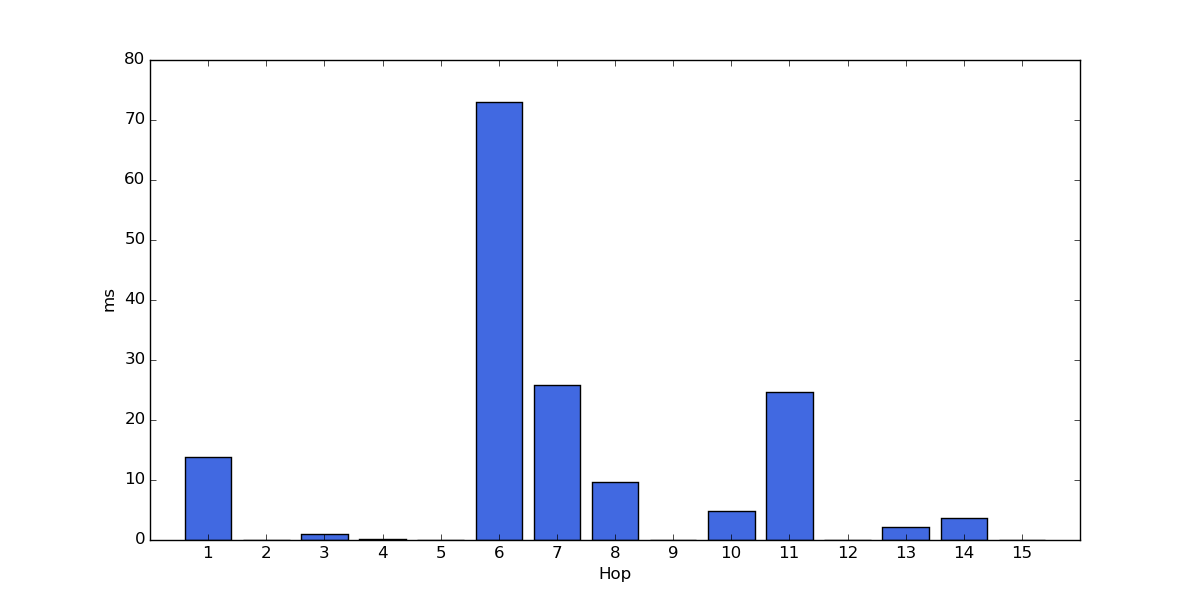
\includegraphics[width=1\textwidth]{data/rtt-malaga-bar.png}
        \caption{www.uma.es - $\Delta$RTT}
        \label{histo:malaga}
    \end{center}
\end{figure}

\begin{figure}[H]
    \begin{center}
        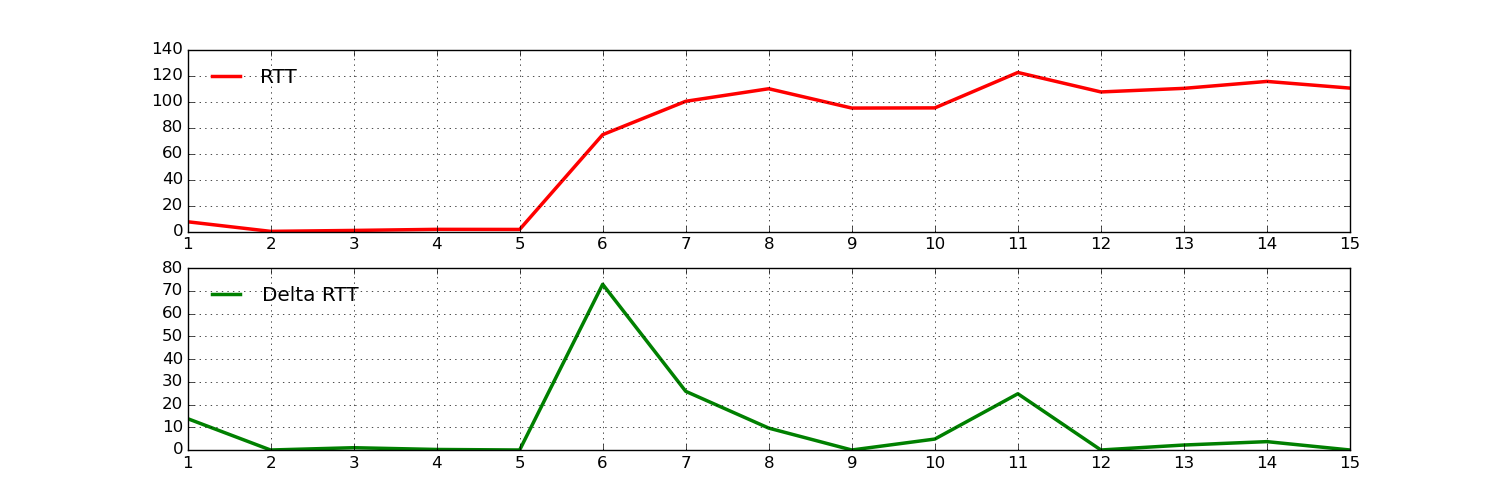
\includegraphics[width=1\textwidth]{data/rtt-malaga-lines.png}
        \caption{www.uma.es - RTT y $\Delta$RTT}
        \label{lines:malaga}
    \end{center}
\end{figure}

Tanto en la figura \ref{histo:malaga} como en la figura \ref{lines:malaga} podemos comprobar los que habíamos notado en la tabla \ref{table:malaga}. El salto 6 se destaca sobre el resto. Es probable que exista un enlace submarino utilizado para ir de América a Europa en ese salto. Esto lo analizaremos en las siguientes secciones.

\subsubsection{Test de Grubbs}\label{malaga:grubbs}

Previo a correr el test de Grubbs corrimos un test de normalidad sobre la distribución de $\Delta$RTT obteniendo los siguientes resultados:

\begin{itemize}
\item \textbf{z-score: 26.158}
\item \textbf{p-value: 0.000}
\end{itemize}

De los resultados obtenidos deducimos entonces que la distribución de los $\Delta$RTT no tiene una distribución Normal, igualmente como mencionamos en la sección \ref{desarrollo:stats} correremos el test de Grubbs a fin de corroborar luego si encuentra los enlaces submarinos de todas formas.\\
Los resultados obtenidos fueron los siguientes outliers:

\begin{itemize}
\item 154.54.31.190
\end{itemize}


\subsubsection{Geolocalización}

\begin{table}[H]
    \begin{center}
        \begin{tabular}{| r | r | c | c |}
  \hline
  {\bf TTL} & \multicolumn{1}{|c|}{\bf IP} & {\bf DNS} & {\bf Ubicación}\\
  \hline
\hline 1 & 45.55.128.253 & no disponible & United States, New York\\
\hline 2 & 162.243.188.221 & no diponible & United States, New York\\
\hline 3 & 62.115.45.9 & nyk-b3-link.telia.net & United States, New York\\
\hline 4 & 154.54.11.109 & be1299.ccr21.jfk04.atlas.cogentco.com & United States, Washington\\
\hline 5 & 154.54.47.29 & be2325.ccr42.jfk02.atlas.cogentco.com & United States, Washington\\
\rowcolor{blue!25}\hline 6 & 154.54.31.190 & be2747.ccr42.par01.atlas.cogentco.com & United States, Washington\\
\hline 7 & 130.117.50.78 & be2423.ccr22.bio02.atlas.cogentco.com & Spain, Bilbao\\
\hline 8 & 130.117.50.26 & be2293.ccr22.mad05.atlas.cogentco.com & Spain, Madrid\\
\hline 9 & 130.117.0.118 & te0-0-2-0.rcr11.b015537-1.mad05.atlas.cogentco.com & Spain, Madrid\\
\hline 10 & 149.11.68.50 & no disponible & Spain, Madrid\\
\hline 11 & 130.206.245.38 & ciemat.ae1.cica.rt1.and.red.rediris.es & Spain, Madrid\\
\hline 12 & 130.206.194.2 & cica-router.red.rediris.es & Spain, Madrid\\
\hline 13 & 150.214.231.2 & xe-0-0-0.malaga01.red.cica.es & Spain, Andalucia, Baeza\\
\hline 14 & 150.214.231.170 & uma-router.red.cica.es & Spain, Andalucia, Baeza\\
\hline 15 & 150.214.40.97 & www.uma.es & Spain, Andalucia, M\'alaga\\
\hline
        \end{tabular}
        \caption{Ruta utilizada para llegar www.uma.es con la ubicación de los diferentes saltos por los que se pasa. Se encuentra resaltado el salto distinguido calculado en la sección \ref{malaga:grubbs}}
        \label{table:malaga} 
    \end{center}
\end{table}

En la tabla \ref{table:malaga} notamos que el salto 6 figura ubicado en Washington, Estados Unidos siendo correctamente el distinguido ya que el siguiente salto figura situado en Europa. En el mapa \ref{mapa:malaga} se puede apreciar el enlace intercontinental. Los saltos 6 y 7 aparecen en el mapa con el nombre de ``B'' y ``C'' respectivamente.


\begin{figure}[H]
    \begin{center}
        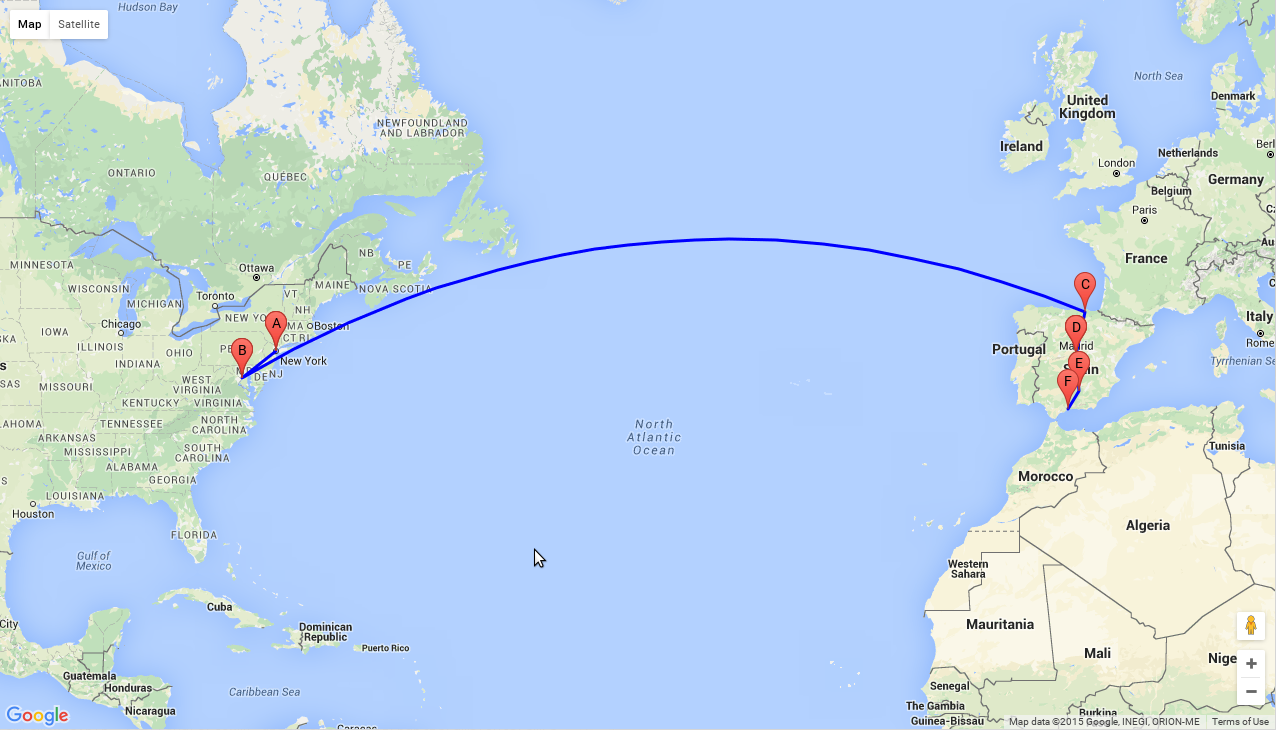
\includegraphics[width=1\textwidth]{data/mapa-malaga.png}
        \caption{www.uma.es - Traceroute}
        \label{mapa:malaga}
    \end{center}
\end{figure}






\subsection{Universidad MIT}
El host de destino fue la universidad M.I.T cuyo dominio es ``web.mit.edu'' con dirección ip ``23.3.254.242''. El server que contiene el sitio se encuentra en Boston, EEUU. El traceroute se originó en Buenos Aires.


\subsubsection{Datos}

Los datos obtenidos para este caso fueron los siguientes:

\begin{table}[H]
    \begin{center}
        \begin{tabular}{| r | r | r | r | r |}
  \hline
  {\bf TTL} & \multicolumn{1}{|c|}{\bf IP} & {\bf E(RTT) (ms)} & {\bf S(RTT) (ms)} & {\bf $\Delta$RTT (ms)}\\
  \hline
\hline 1 & 36.6.64.1 & 16.857 & 19.297 & 16.857 \\
\hline 2 &  190.220.185.65 & 14.007 & 8.700 & 0.000   \\
\hline 3 &  10.2.8.205 & 16.958 & 17.230 & 2.951   \\
\hline 4 &  10.2.11.217 & 19.137 & 13.277 & 2.179   \\
\hline 5 &  10.2.11.217 & 18.659 & 15.835 &  0.000   \\
\hline 6 &  10.2.11.229 &  17.837   &  10.482   &  0.000   \\
\hline 7 &  10.2.11.229 & 18.594   &  11.833   &  0.758   \\
\rowcolor{blue!25}\hline 8 & 208.48.239.69 & 155.411   & 63.920   &  136.817   \\
\hline 9 &  4.69.207.38 & 143.480   & 7.582    &  0.000   \\
\hline 10 &  4.69.132.114 & 175.854   & 17.489   &  32.374   \\
\hline 11 &  4.69.140.133 & 175.043   & 15.968   &  0.000   \\
\hline 12 &  4.69.151.161 & 173.678   & 21.824   &  0.000   \\
\hline 13 &  4.69.145.209 & 172.987   & 14.266   &  0.000   \\
\hline 14 &  4.59.36.26 & 175.472   & 15.564   &  2.485   \\
\hline 15 &  94.142.125.70 & 208.940   & 20.446   &  33.468   \\
\rowcolor{blue!25}\hline 16 & 94.142.124.33 & 303.767   & 24.269   &  94.828   \\
\hline 17 &  5.53.1.26 & 302.054 & 23.695   &  0.000   \\
\hline 18 &  120 & 0.000 & 0.000 &  0.000   \\
\rowcolor{blue!25}\hline 19 & 186.148.62.33 & 303.300   & 17.808   &  303.300   \\
\rowcolor{blue!25}\hline 20 &  186.148.62.34 & 349.613   & 63.907   &  46.313   \\
\hline 21 &  23.3.254.242 & 303.657   & 18.741   &  0.000   \\
\hline
        \end{tabular}
        \caption{$\overline{RTT}$, $\sigma$RTT y $\Delta$RTT para la ruta utilizada para llegar a web.mit.edu}
        \label{table:mit} 
    \end{center}
\end{table}


\subsubsection{RTT y $\Delta$RTT}

\begin{figure}[H]
    \begin{center}
        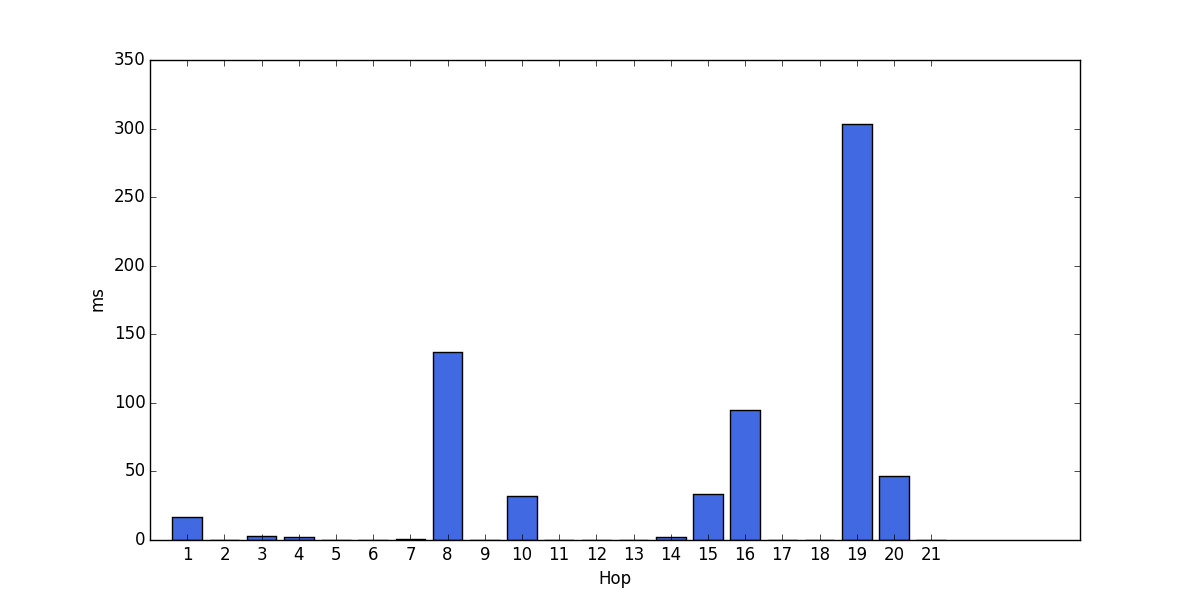
\includegraphics[width=1\textwidth]{data/rtt-mit-bar.png}
        \caption{web.mit.edu - $\Delta$RTT}
        \label{histo:mit}
    \end{center}
\end{figure}

\begin{figure}[H]
    \begin{center}
        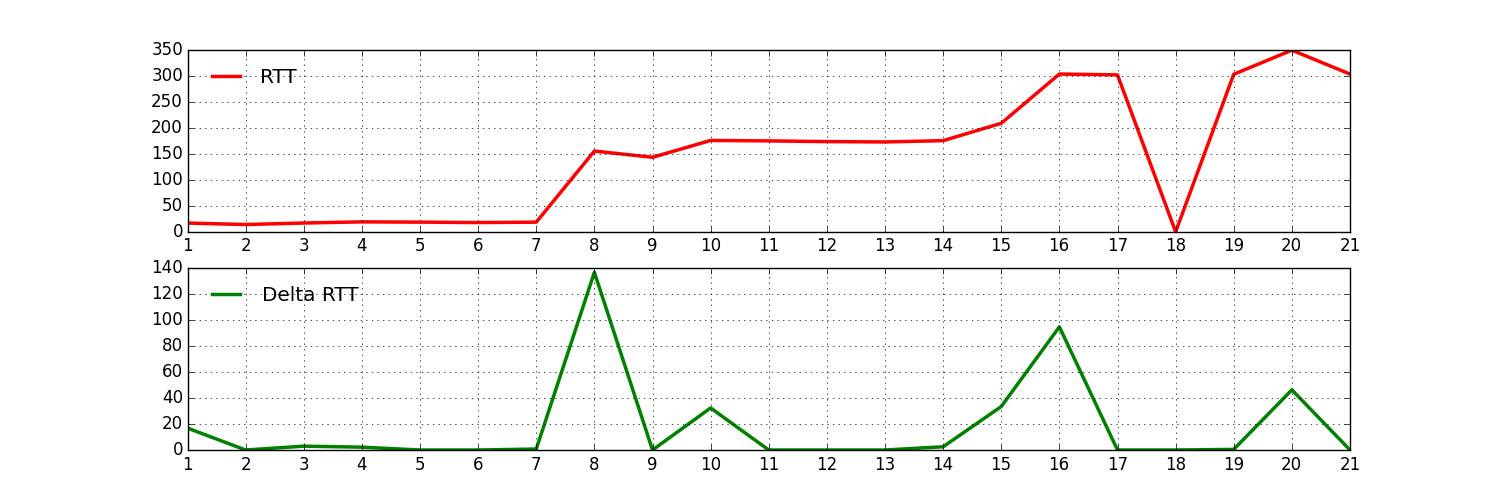
\includegraphics[width=1\textwidth]{data/rtt-mit-lines.png}
        \caption{web.mit.edu - RTT y $\Delta$RTT}
        \label{lines:mit}
    \end{center}
\end{figure}


Podemos ver en las figuras \ref{table:mit}, \ref{histo:mit} y en el cuadro \ref{lines:mit} que el $\Delta$RTT correspondiente a los $TTL$ $8$, $16$, $19$ y en menor medida $21$, son mas grande que el resto. En las siguientes secciones se analizará si estos corresponden a transmiciones por enlaces submarinos.


\subsubsection{Test de Grubbs}\label{mit:grubbs}

Previo a correr el test de Grubbs corrimos un test de normalidad sobre la distribución de $\Delta$RTT obteniendo los siguientes resultados:

\begin{itemize}
\item \textbf{z-score: 35.795}
\item \textbf{p-value: 0.000}
\end{itemize}

De los resultados obtenidos deducimos entonces que la distribución de los $\Delta$RTT no tiene una distribución Normal, igualmente como mencionamos en la sección \ref{desarrollo:stats} correremos el test de Grubbs a fin de corroborar luego si encuentra los enlaces submarinos de todas formas.\\
Los resultados obtenidos fueron los siguientes outliers:

\begin{itemize}
\item 186.148.62.33
\item 208.48.239.69
\item 94.142.124.33
\item 186.148.62.34
\end{itemize}


\subsubsection{Geolocalización}

\begin{table}[H]
    \begin{center}
        \begin{tabular}{| r | r | c | c |}
  \hline
  {\bf TTL} & \multicolumn{1}{|c|}{\bf IP} & {\bf DNS} & {\bf Ubicación}\\
  \hline
\hline 1 & 36.6.64.1 & no disponible & China, Hefei\\
\hline 2 & 190.220.185.65 & no disponible & Argentina, Berazategui\\
\hline 3 & 10.2.8.205 & no disponible & no disponible\\
\hline 4 & 10.2.11.217 & no disponible & no disponible\\
\hline 5 & 10.2.11.217 & no disponible & no disponible\\
\hline 6 & 10.2.11.229 & no disponible & no disponible\\
\hline 7 & 10.2.11.229 & no disponible & no disponible\\
\rowcolor{blue!25}\hline 8 & 208.48.239.69 & 7-2-34.ear4.Miami2.Level3.net & United States, Lawrenceville\\
\hline 9 & 4.69.207.38 & no disponible & United States, Kansas\\
\hline 10 & 4.69.132.114 & no disponible & United States, Kansas\\
\hline 11 & 4.69.140.133 & ae-2-2.ebr1.Dallas1.Level3.net & United States, Hialeah\\
\hline 12 & 4.69.151.161 & ae-91-91.csw4.Dallas1.Level3.net & United States, Dallas\\
\hline 13 & 4.69.145.209 & ae-4-90.edge5.Dallas3.Level3.net & United States, Dallas\\
\hline 14 & 4.59.36.26 & TELEFONICA.edge5.Dallas3.Level3.net & United States, Kansas\\
\hline 15 & 94.142.125.70 & no disponible  & España\\
\rowcolor{blue!25}\hline 16 & 94.142.124.33 & no disponible & España\\
\hline 17 & 5.53.1.26 & no disponible & España\\
\hline 18 & * & no disponible & no disponible\\
\rowcolor{blue!25}\hline 19 & 186.148.62.33 & akamai.Vl366.lflo.internacional.pe.nap.movistar.cl  & Chile, Santiago\\
\rowcolor{blue!25}\hline 20 & 186.148.62.34 & akamai.Vl366.lflo.internacional.ce.nap.movistar.cl & Chile, Santiago\\
\hline 21 & 23.3.254.242 & 242.deploy.static.akamaitechnologies.com & United States, Cambridge\\
\hline
        \end{tabular}
        \caption{Ruta utilizada para llegar web.mit.edu con la ubicación de los diferentes saltos por los que se pasa. Se encuentran resaltados los saltos correspondientes a outliers encontrados con el test de Grubb}
        \label{table:mit} 
    \end{center}
\end{table}

En el cuadro \ref{table:mit} se observa que los saltos distinguidos corresponden a enlaces submarinos. Podemos notar que el primer salto ocurre a un servidor que nuestras herramientas de geolocalización sitúan en China, pero si notamos el rtt hacia el mismo, es probable que la localización sea errónea. Luego de investigar esa ip, nos dimos cuenta que, realizando traceroutes hacia servidores que se encuentran en Argentina, la ip 36.6.64.1 aparece igualmente, lo que, aunque no es imposible, tiene poco sentido si el servidor realmente se encuentra en China. \\
    Teniendo en cuenta esto, el rtt bajo y el hecho de que rutas hacia servidores en  argentina también pasan por dicha ip, creemos que el servidor correspondiente pertenece a alguna red interna del ISP (Claro en este caso), posiblemente con alguna mala configuración.


\begin{figure}[H]
    \begin{center}
        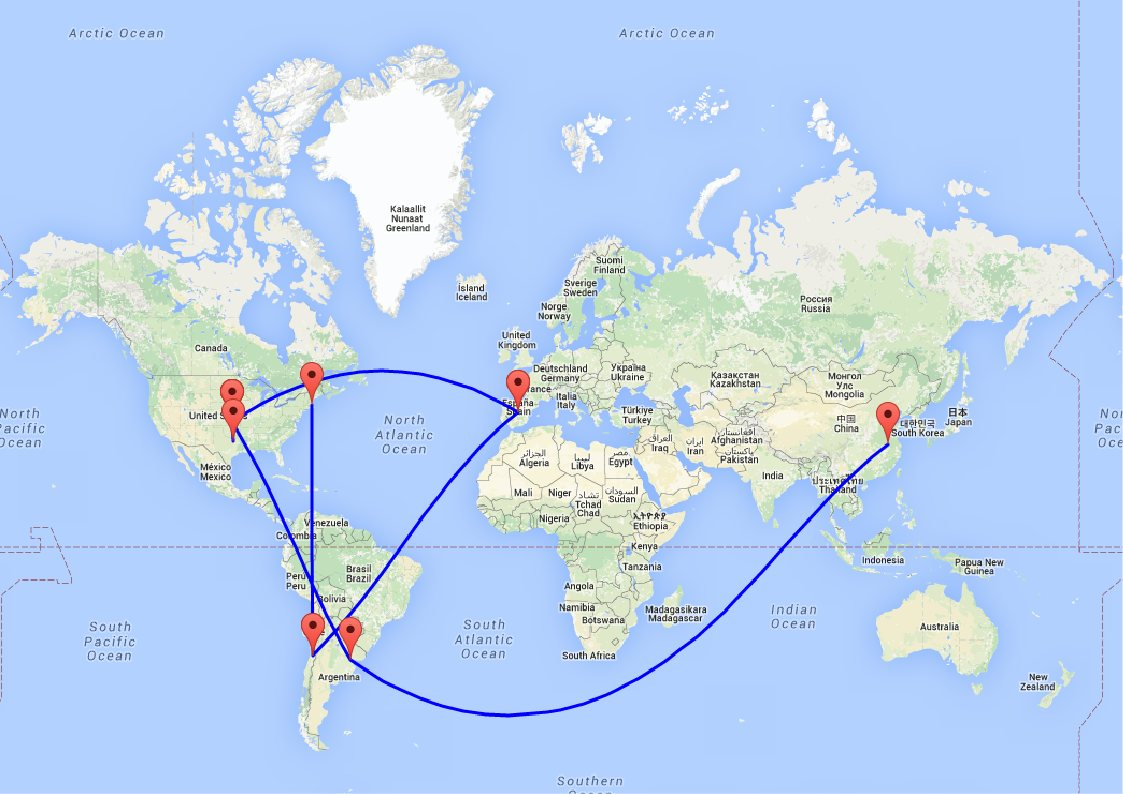
\includegraphics[width=1\textwidth]{data/mapa-mit.jpg}
        \caption{web.mit.edu - Traceroute}
        \label{mapa:mit}
    \end{center}
\end{figure}

Vemos, nuevamente, en la figura \ref{mapa:mit} que los outliers encontrados corresponden a enlaces submarinos.

